\subsection{Prototype Simulations}
\label{sec:prototypeSimulations}

\textbf{\underline{Signal Homogeneity across a Scintillator Tile}}

In this simulation the signal homogeneity across a scintillator tile was investigated, i.e. to what extend the number of photons that reach the photon detector depends on the position at which a minimum ionising particle (MIP) hits the scintillator tile. Four different set-ups have been simulated: 100$\times$100$\times$5$\,$mm$^3$ and 350$\times$350$\times$5$\,$mm$^3$ scintillator tiles (BC-408) with Teflon wrapping and readout via one pseudo-SiPM, which was either attached directly to the tile or by an embedded wavelength-shifting fibre (cf. figure\enspace\ref{fig:simulatedSetups}). In case of the wavelength-shifting fibre, the end inside the scintillator has been mirrored and a pseudo-SiPM has been placed at the other end. For each of the four set-ups, 100000 MIP muons have been simulated randomly distributed over the scintillator surface, to obtain reasonable statistics.

\begin{figure}[h]
  \centering
  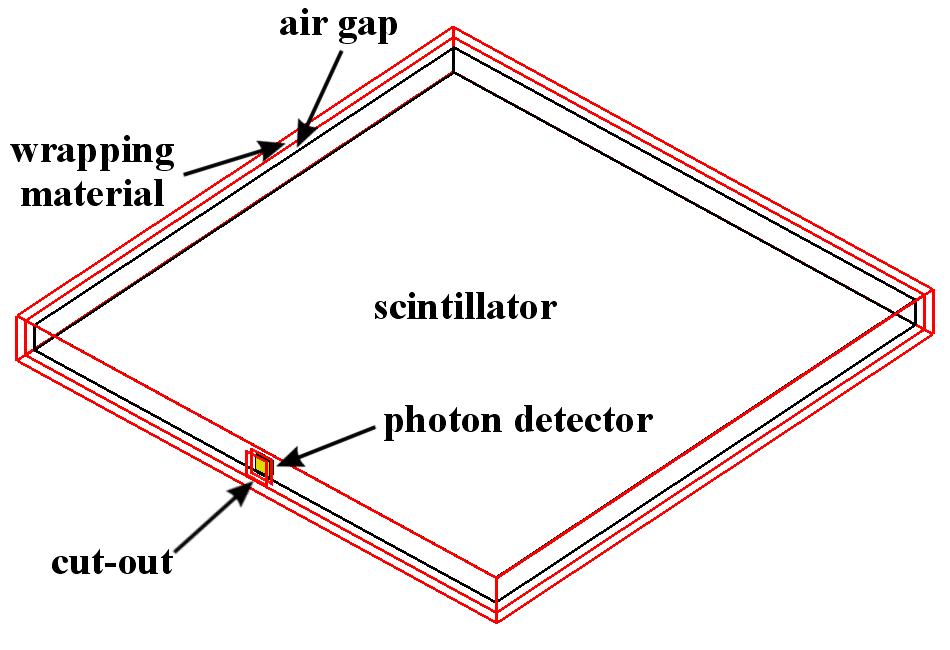
\includegraphics[width=8.9cm]{Figures/dietzlaursonn/wrapping.png}
  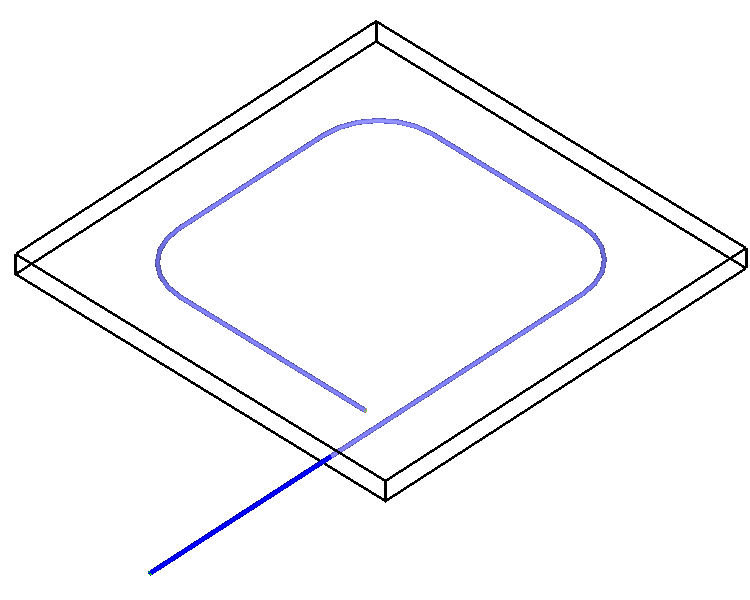
\includegraphics[width=7cm]{Figures/dietzlaursonn/fibre_sigma.png}
  \caption{\textbf{Left:} Set-up consisting of a wrapped scintillator tile with a photon detector. To make them visible, the dimensions of the wrapping as well as the free space between photon detector and wrapping, or scintillator and wrapping have been set to large values when generating the picture. \textbf{Right:} Relatively complex fibre set-up within and extending a scintillator tile.}
  \label{fig:simulatedSetups}
\end{figure}

In the following plots, the $x$- and $y$-axes represent the position at which the muons hit the scintillator tile. The colour-coded $z$-axis shows the most probable value (MPV) of the number of photons hitting the pseudo-SiPM. The MPV has been obtained by a fit of a Landau distribution to the distribution of the number of photons for the corresponding position bin. Since the energy deposition of a particle in thin layers of matter follows a landau distribution, no meaningful mean and standard deviation can be computed. As uncertainty on the number of photons, the uncertainty of the MPV of the fitted Landau distribution is taken. It is on average below 5\% across the tiles and below 10\% next to the SiPMs for direct readout.

Figure\enspace\ref{fig:signalHomogeneity} shows the signal homogeneity for all four simulated set-ups. For direct readout, the signal is relatively homogeneous over large areas and with values of MPV $\approx 550$ or MPV $\approx 50$ photons, depending on the dimensions of the scintillator tile. But in cases of muons that hit the scintillator tile in short distance to the pseudo-SiPM, the number of photons that reach the pseudo-SiPM increases dramatically by factors up to $\approx 5$ or $\approx 8$, depending on the dimensions of the scintillator tile. Such a signal inhomogeneity across the scintillator tile can be very problematic e.g. for the determination of the MIP muons. Additionally, depending on its number of pixels, an SiPM would probably be saturated and not able to detect multiple muon hits within a short time.

Using wavelength-shifting fibres to collect the scintillation light and to guide it to the pseudo-SiPM can significantly reduce this effect. This is illustrated in the bottom plots of figure\enspace\ref{fig:signalHomogeneity}. 
The signal is relatively homogeneous over the whole area with values of MPV $\approx 280$ or MPV $\approx 120$ photons, depending on the dimensions of the scintillator tile. In small distance to the fibre, the number of photons that reach the pseudo-SiPM increases, but only by $\approx 15\%$ or $\approx 60\%$, depending on the dimensions of the scintillator tile.

\begin{figure}[h]
\centering
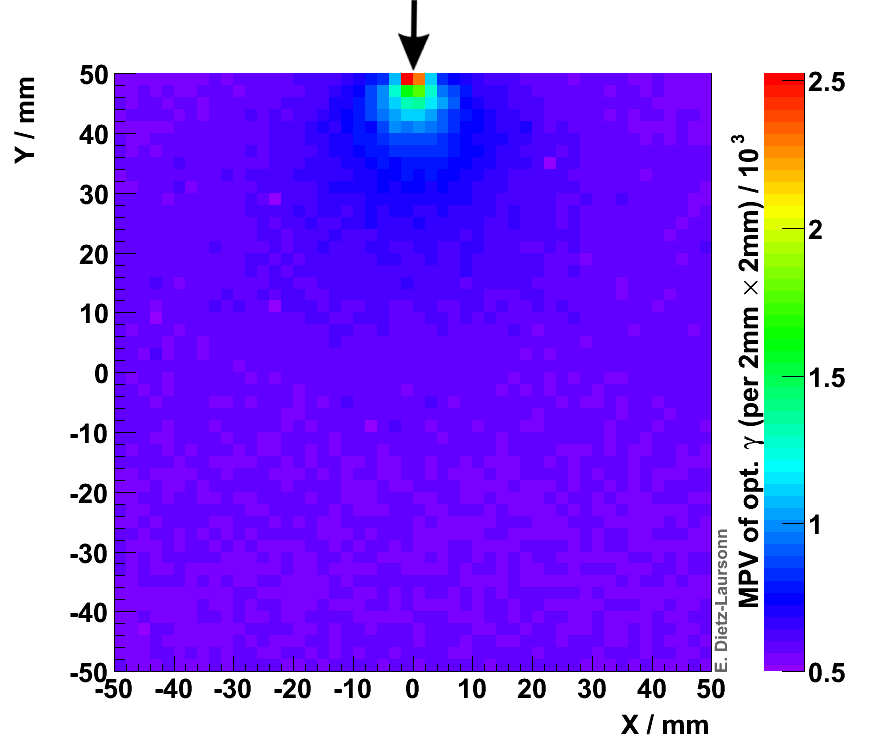
\includegraphics[width=7.9cm]{Figures/dietzlaursonn/101_100x5x100_Teflon__dataSim_opticalPhotons_on_SiPM_vs_hit_position.png}
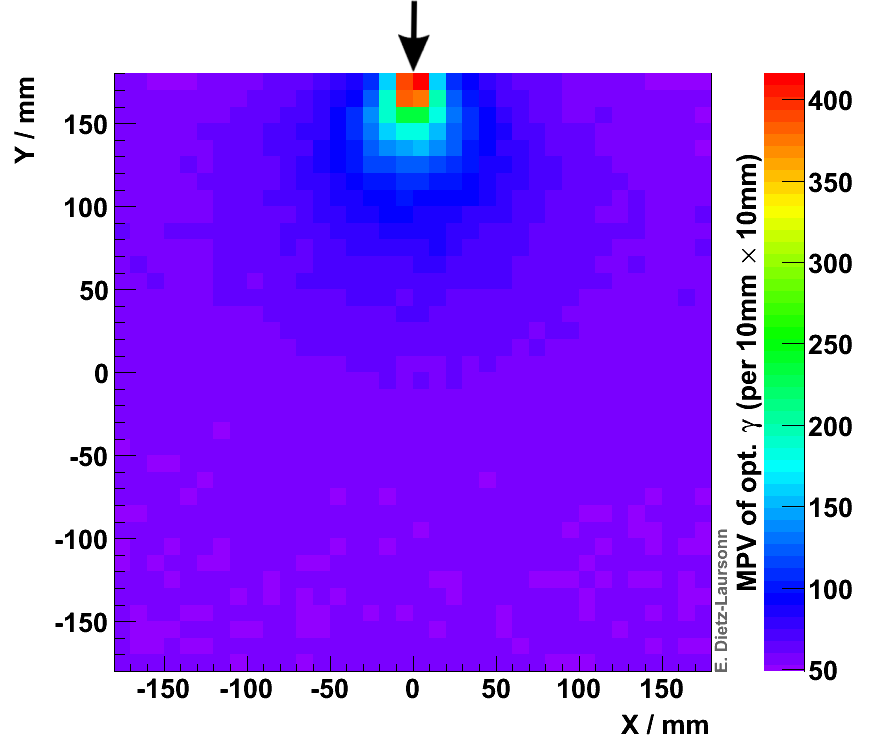
\includegraphics[width=7.9cm]{Figures/dietzlaursonn/101_350x5x350_Teflon__dataSim_opticalPhotons_on_SiPM_vs_hit_position.png}

\vspace{0.5cm}
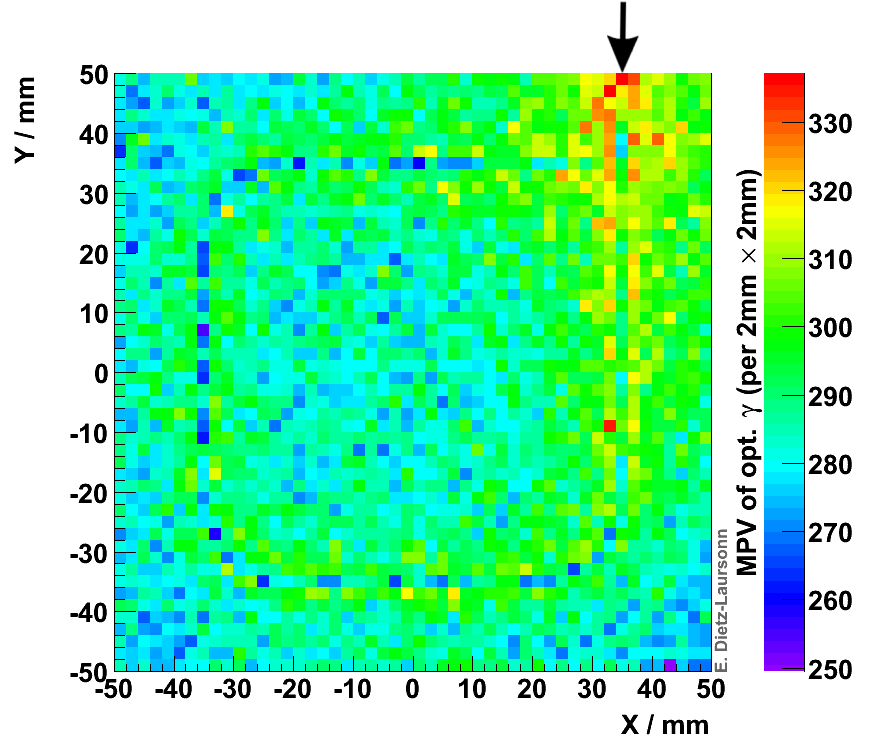
\includegraphics[width=7.9cm]{Figures/dietzlaursonn/411_100x5x100_Teflon__dataSim_opticalPhotons_on_SiPM_vs_hit_position.png}
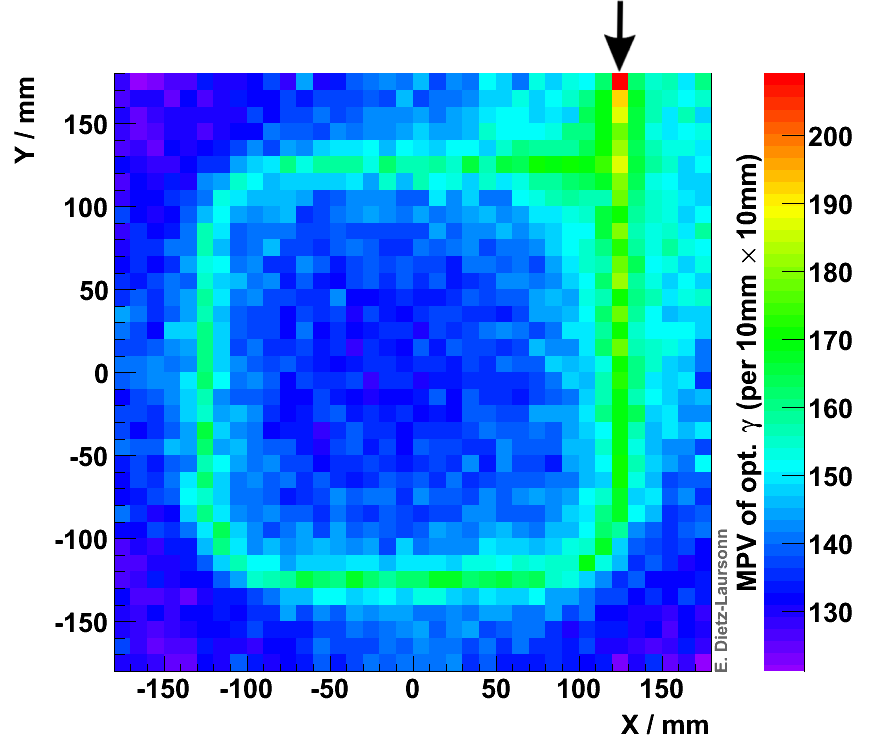
\includegraphics[width=7.9cm]{Figures/dietzlaursonn/411_350x5x350_Teflon__dataSim_opticalPhotons_on_SiPM_vs_hit_position.png}
\caption{Signal homogeneity for all four simulated set-ups: \textbf{Top-left:} 100$\times$100$\times$5$\,$mm$^3$ scintillator tile with direct readout, \textbf{Top-right:} 350$\times$350$\times$5$\,$mm$^3$ scintillator tile with direct readout, \textbf{Bottom-left:} 100$\times$100$\times$5$\,$mm$^3$ scintillator tile with fibre readout, \textbf{Bottom-right:} 350$\times$350$\times$5$\,$mm$^3$ scintillator tile with fibre readout. The arrows indicate the SiPM positions.}
\label{fig:signalHomogeneity}
\end{figure}




\textbf{\underline{Validation with hodoscope measurements}}

As validation, the results of the simulation have been compared to measurements that have been performed with a prototype detector tile within a hodoscope. The prototype detector tile consist of  a 100$\times$100$\times$5$\,$mm$^3$ scintillator tile (BC-408) with Teflon wrapping and two SiPMs. Both SiPMs are coupled to the scintillator tile at one of its thin surfaces, at a distance of 2$\,$cm with respect to the centre position. The data acquisition of the SiPM signal has been performed via a Charge-to-Digital-Converter.

The hodoscope consist of two layers of two vertical Silicon-Strip-Detectors each. They provide two positions (and thus the trajectory) of  cosmic muons and therefore allow the determination of the muon's hit position on the prototype detector tile, which is placed between the two hodoscope layers.

Up to now, 8436 cosmic muon tracks could be recorded and measured by the SiPMs.



In the following plots, the $x$- and $y$-axes again represent the position where the muons hit the scintillator tile. The uncertainties on the measured hit position on the scintillator tile are negligible in comparison to the used bin width. The relatively large bin width is due to the low statistics.
The colour-coded $z$-axis shows the difference between measured and simulated MPV. Since the measurement results in the MPV of the SiPM signal charge, only relative values can be compared. Therefore, the original MPV values have been scaled to the mean value of the marked comparison area and the resulting relative values were used to determine the difference between measurement and simulation. The uncertainties shown in the histograms are the propagated MPV uncertainties of the fitted Landau distributions for both, the simulation and the measurement.



\begin{figure}[h]
\centering
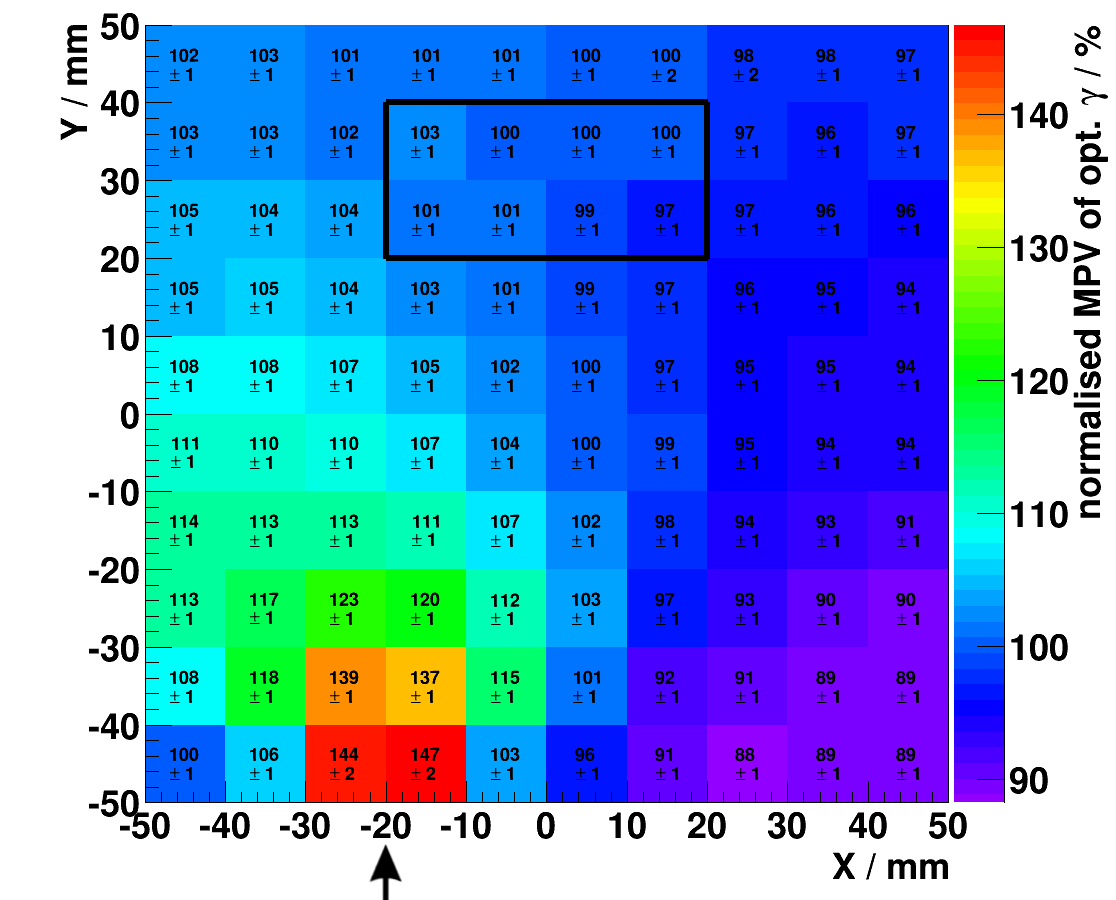
\includegraphics[width=7.9cm]{Figures/dietzlaursonn/comparison_sim_B_opticalCoupling_1_43_1cm.png}
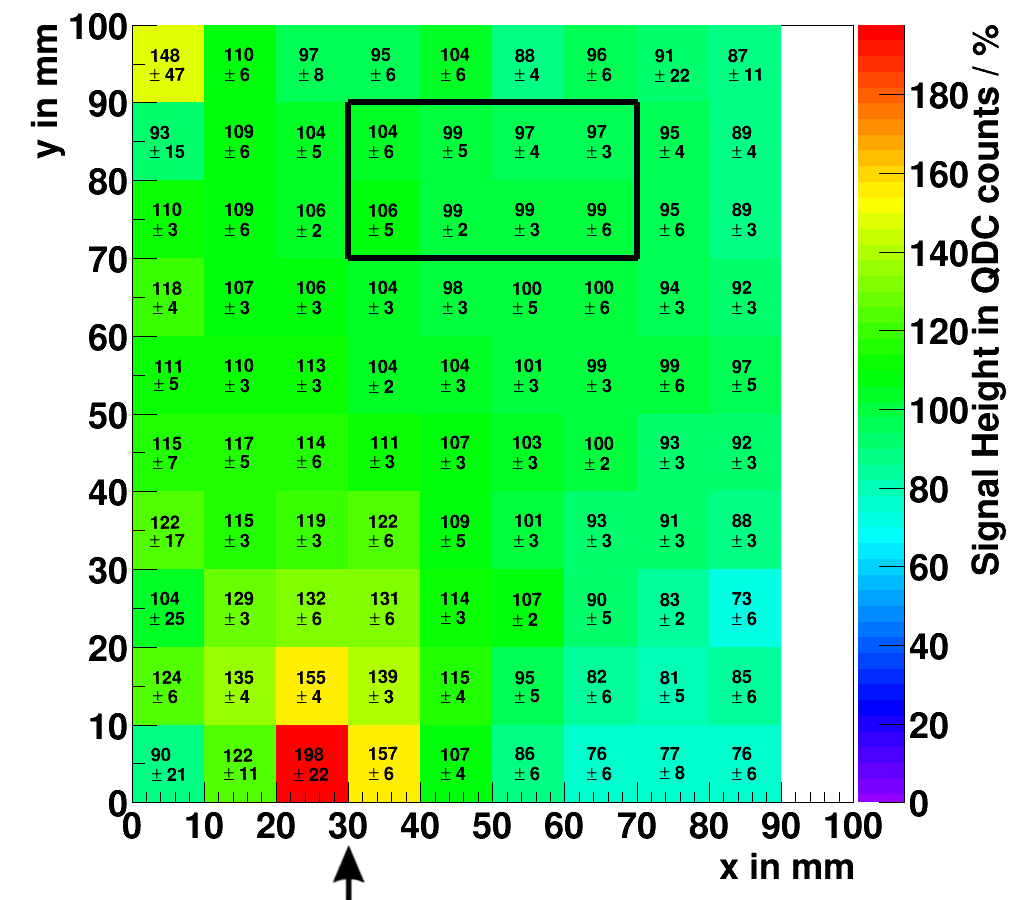
\includegraphics[width=7.9cm]{Figures/dietzlaursonn/comparison_meas_B_1cm.png}

\vspace{0.5cm}
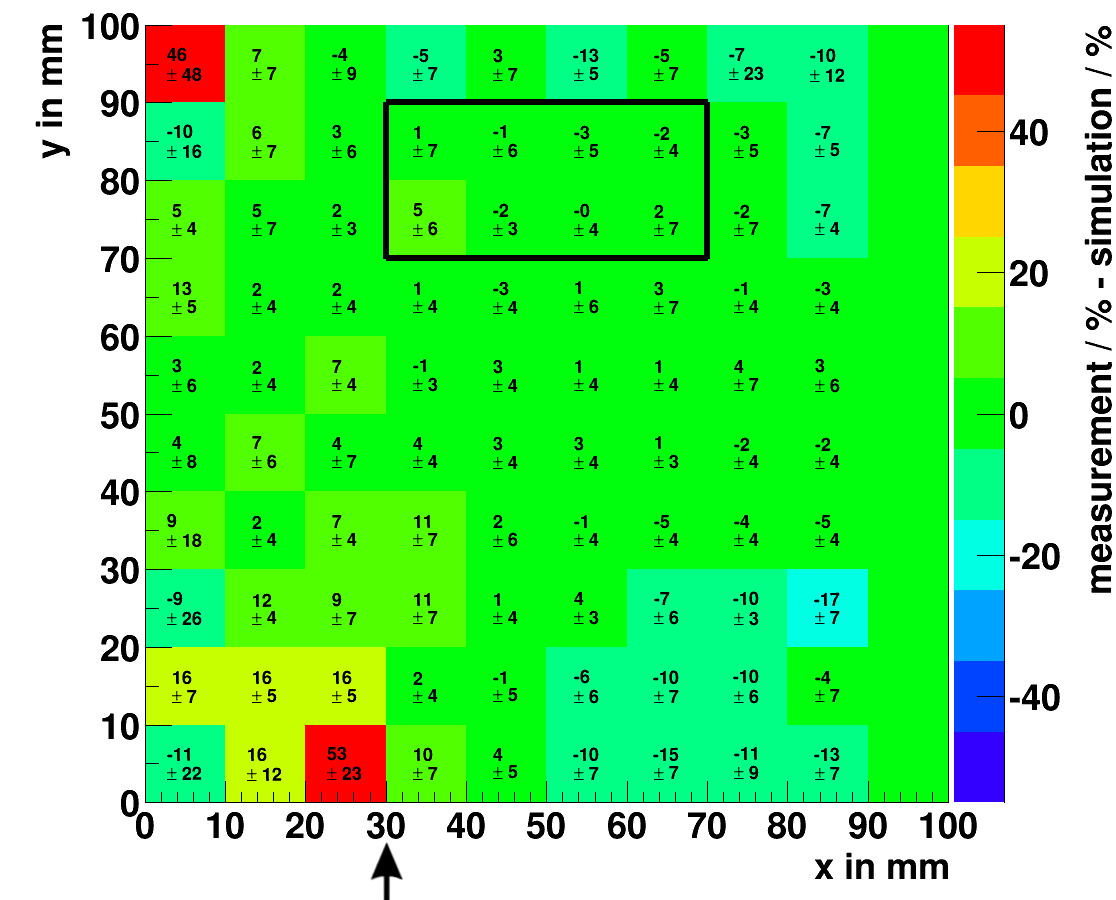
\includegraphics[width=8cm]{Figures/dietzlaursonn/comparison_diff_B_opticalCoupling_1_43_1cm.png}
\caption{Results for the comparison between measurement and simulation: \textbf{Top-left:} normalised simulation results, \textbf{Top-right:} normalised measurement results (the unfilled bins were caused by the geometry of the hodoscope), \textbf{Bottom:} the difference between simulation and measurement. The arrows indicate the SiPM position and the results have been been scaled to the mean value of the marked comparison area.}
\label{fig:comparison}
\end{figure}



Figure\enspace\ref{fig:comparison} illustrates the scaled results of the simulation and the measurement as well as the difference between them. Again, the signal is relatively homogeneous over large areas and dramatically increases next to the SiPM position. The comparison shows, that the relative distribution of simulation and measurement are in very good agreement and the difference is compatible with 0 over a large area, when considering the uncertainties. As repeating the measurement after reassembling the detector reproduces the MPV values with 10\% accuracy, which is caused by the limited reproducibility of the optical coupling between scintillator tile and SiPM, the achieved agreement between simulation and measurement is an excellent result.

